\documentclass[11pt]{article}
\usepackage{geometry}                % See geometry.pdf to learn the layout options. There are lots.
\geometry{letterpaper}                   % ... or a4paper or a5paper or ... 
%\geometry{landscape}                % Activate for for rotated page geometry
%\usepackage[parfill]{parskip}    % Activate to begin paragraphs with an empty line rather than an indent
\usepackage{graphicx}
\usepackage{amssymb}
\usepackage{epstopdf}
\usepackage{amsmath}
\usepackage{graphicx}
\graphicspath{{images/}}
\usepackage{float}
\usepackage{wrapfig}
\usepackage[titletoc, title]{appendix}
%\DeclareMathOperator{\sinc}{sinc}

\DeclareGraphicsRule{.tif}{png}{.png}{`convert #1 `dirname #1`/`basename #1 .tif`.png}

\title{Application of Compressive Sensing to Simulated Chemical Spectra}
\author{Camille Houferak, Joe Kasper, Joseph J. Radler, Shichao Sun}
\date{\today}                                           % Activate to display a given date or no date

\begin{document}
\maketitle
\begin{abstract}

Abstract

\end{abstract}

% SECTION I -- INTRODUCTION AND OVERVIEW

\section*{I.	Introduction and Overview}  %J will write this

%\begin{wrapfigure}{r}{0.38\textwidth}
%Sets wrapped figure to the right of the page
%\includegraphics[width=2.5in]{derek1}
%\caption{Corrupted Image of Derek's Trademark Look}
%\end{wrapfigure}

\par Computational chemistry seeks to construct fine-grained models of chemical systems in order to model and predict experimentally observable quantities in support of experimental research.  A major implementation of computational modeling is the construction of idealized chemical spectra, which are essentially the 'fingerprints' of a chemical species in a system of interest.  Traditionally, spectra have been generated experimentally, but recently have been generated from models of molecular electronic structure which comprises a major field of study in the computational chemistry community.  However, generating predictive spectra from model and simulation can be a difficult undertaking, as the number of degrees of freedom for a so-called \emph{full configuration} solution increases exponentially (or factorially!) for each additional electron found in the system. Full configuration calculations are ideal for capturing \emph{all} of the physics of a system, but come at great computational expense as every interaction between each particle must be accounted for in the Hamiltonian and the second-order differential \emph{Schr\"odinger Equation} solved numerically.  If atomic nuclear dynamics are also modeled, this increases the complexity even further as each solution for each time step.  Consequently, approximations and calculation schemes that minimize the complexity and computational cost of a model are highly valued in the field. Accordingly, techniques for reducing or removing the necessity of small time-steps and long timescales are also of great utility, as dynamical simulations examining nuclear motion often require picosecond timescales to capture the physics of interest whereas models examining only electronic dynamics require only femtosecond timescales.\\ 

\par Things are not so bleak, however, as there is an abundance of mathematical techniques for reducing the scale of such problems. This study focuses on one such technique called \emph{Compressed Sensing} (CS) that is used in data analysis to reduce the necessary sampling rate. CS does this by assuming a high degree of sparsity in a signal and makes use of the $L^{1}$ norm minimization technique to locate the vector of signal transform coefficients that is the most sparse.  As CS is frequently applied to time-frequency analysis problems, we apply it to modeled chemical spectra which heavily feature Fourier analysis for signal resolution.  This particular investigation focuses on \emph{Optical Absorption Spectroscopy} -- an electronic process in molecular systems where electrons are excited to higher discrete quantum states upon absorption of incident photons. \\ 
 
\par Modeling absorption spectra computationally presents a unique challenge since the propagation of electronic states through time is the fundamental process behind the generation of experimentally observable spectra.  Several schemes exist for performing calculations that capture electron dynamics, however here we focus only on simulated spectra obtained through a \emph{Real-Time Time-Dependent Density Functional Theory} (RT-TDDFT) scheme which solves electron dynamics by self-consistently solving a set of pseudoeigenvalue equations of electronic wavefunctions for each iteration in time, then solving an electron density functional equation based on those wavefunctions.  The calculations are performed while holding the nuclear positions fixed (using the \emph{Born-Oppenheimer approximation}) in order to reduce the number of degrees of freedom in the system of interest.  As one can imagine, this can become prohibitively expensive for large systems with many electrons or large numbers of time steps; therefore we seek to find the best CS sampling rate to reduce the number of necessary time steps to achieve satisfactory optical absorption spectral resolution for molecular systems. In principle we can generalize this technique for other simulated chemical spectra.\\

\par This investigation divides the examination of compressed sensing into two parts.  \emph{Part One} compares the output of the Fast Fourier Transform (FFT) of our sampling subset with the, Discrete Sine Transform (DST) within the CS algorithm to an idealized, known linear combination of sinusoidal functions representing our absorption signal.  \emph{Part Two} explores the application of CS to simulated optical absorption spectra for water obtained by RT-TDDFT calculations of electric dipole oscillations.  The $L^{1}$ norm minimization is carried out using the SPGL$_{1}$  algorithm as implemented in MATLAB (see \emph{Appendix A}) and all code is implemented in MATLAB (see \emph{Appendix B}).

% SECTION II -- THEORETICAL BACKGROUND

\section*{II.	Theoretical Background}	%J and Camille	
\subsection*{A.	An Introduction to Optical Absorption Spectroscopy} %Camille

\par Spectroscopy is a useful and highly utilized technique throughout the field of chemistry that investigates how a molecule or material interacts with electromagnetic radiation. One commonly used form of this general technique is that of optical absorption spectroscopy, wherein light is used as a probe of the properties and functionalities of compounds. In UV-visible spectroscopy (UV-vis), for example, a sample is exposed to light in the ultraviolet and visible range of wavelength. When a particular wavelength corresponds with the energy gap between energy levels of the molecule, electrons can be excited into higher energy molecular orbitals. A typical spectrum in this technique will plot absorbance as a function of wavelength, where absorbance is given by:

\begin{align}\label{eq:abs}
A = \log_{10}{(I_0/I)}
\end{align}

where I$_0$ is the intensity of the incident light and I is the intensity of the light after passing through a sample. Thus, for a range of wavelengths, spectra will show peaks at wavelengths which correspond to light being absorbed to excite an electron to a different energetic state. One can see how modeled data of such a spectrum lends itself well to the compressive sensing technique. Although this will be further discussion in section C, have absorbance features for only a few wavelengths will translate to there being sparsity in any matrix representing absorption spectroscopy data. 

\subsection*{B.	Real-Time Time-Dependent Density Functional Theory (RT-TDDFT)} %J 

\par The simulated spectra to which we apply CS in this investigation were generated from a \emph{Real-Time Time-Dependent Density Functional Theory} (RT-TDDFT) calculation. To explain this, some background is needed. Essentially, electrons can be considered to exist as waves around an atomic nucleus in what are known as \emph{wavefunctions}.  When multiple atoms are bonded together, the single electron atomic wavefunctions are summed as a linear combination to form molecular wavefunctions (also called \emph{spin orbitals}.) Molecular spin orbitals may be combined with those of electrons with antiparallel spin to form \emph{spatial orbitals} which, when the modulus squared is taken represent the probability of finding an electron in that region of space about a nucleus.\\

\par Density Functional Theory is based on a theorem called the Hohenberg-Kohn theorem, the first part of which shows that for all electron density functions there exists a unique energy functional corresponding to each density state.  The wavefunctions (or orbitals) come into play when we consider the density of electrons around the nucleus to be a function of the electronic \emph{wavefunction}.  We use idealized, variationally optimized electron wavefunctions called \emph{Kohn-Sham orbitals} to calculate the density from which the energy functional is calculated. However, the exact form of the unique energy functional is unknown in the general case, so quantities that contribute to the overall energy such as electronic exchange (the energy necessary to exchange the positions of two electrons of antiparallel spins) and the electron correlation energies must be corrected to obtain an accurate calculation.  In most DFT methodologies, the first principles (\emph{ab initio}) energy functional is corrected at each point in space by an \emph{Exchange Correlation functional} which is typically a semiempirical correction which accounts for artifacts in the kinetic and electronic exchange terms.\\

\par Time-Dependent Density Functional Theory (TDDFT) then takes the system of interest and calculates the energy functional for each individual time step, then propagates it in time by applying a unitary operator to the density matrix (which describes the electron density for the entire system) with the end goal of resolving electronic dynamics for the system over a given simulation time.  What \emph{Real-Time} TDDFT does is propagate the density matrix according to the TDDFT equation
\begin{equation}\label{eq:tddft}
	i\frac{d\mathbf{P}(t)}{dt} = [\mathbf{K}(t), \mathbf{P}(t)]
\end{equation}
where the right side of the equation is a commutator, $\mathbf{K}(t)$ is the Kohn-Sham matrix, and $\mathbf{P}(t)$ is the density matrix.  Matrix $\mathbf{K}(t)$ is obtained by projecting the previously mentioned Kohn-Sham orbital wavefunctions (eigenstates) onto a space spanned by a set of supporting functions. Subsequently, the electron dynamics are simulated in real-time by propagating the \emph{density matrix} using a unitary time-evolution operator $\mathbf{U}(t_{n})$ expressed in the same eigenbasis as the Kohn-Sham matrix operator at time $t$.  The time evolution can be expressed as, for 

\begin{equation}\label{eq:prop}
\begin{split}
	\mathbf{U}(t_{n}) = exp[-i \cdot\Delta t \cdot \mathbf{K}(t_{n})]\\
	=\mathbf{C}(t_{n})\cdot[-i\cdot\Delta t \cdot \epsilon (t_{n})]\cdot \mathbf{C}^{\dag}(t_{n})
\end{split}
\end{equation}

where

\begin{equation}\label{eq:evol}
	\mathbf{P}(t_{n+1}) = \mathbf{U}(t_{n})\cdot\mathbf{P}(t_{n-1})\cdot\mathbf{U}^{\dag}(t_{n}).
\end{equation}

\par From the density matrix for each iteration, our transition dipole moment data (and pattern of oscillation with respect to time) is calculated and tabulated using the electron density function.  This is the source of the data we use in this investigation into compressive sensing.

\subsection*{C.	Compressive Sensing}	%Joe

\par Traditional methods of time-frequency analysis such as the Fourier transform require that one gathers enough data to exceed the Nyquist rate. However, in the spirit of other dimensional reduction algorithms, there are many signals of interest that are sparse. That is there exists a ``best" simple representation. In particular, we posit \textit{a priori} that only a small number of Fourier coefficients are nonzero. If this is the case, then the task of finding the Fourier coefficients can be greatly simplified. \\

\par Consider a signal $h(t)$ that is sampled $n$ times with a spacing $\Delta t$. Then we may write the signal observations as a vector $\vec{h}$ with $n$ components $h_{j}$ corresponding to the times $t_{j}$. The set of Fourier coefficients that we wish to find for a set of frequencies $\omega_{k}$ are given by $g_{k}$ where $k \in \{1,...,N\}$ and $\Delta \omega$ is constant. In general the $g_{k}$ can be calculated by the discrete sine transform (or any other Fourier transform):

\begin{equation}\label{eq:dst}
    g_{k} = \sum_{j=1}^{n} \Delta t \sin(\omega_{k}t_{j})h_{j}
\end{equation}

Casting this in matrix form, a Fourier matrix $F$ is given by
\begin{equation}\label{eq:idst}
    F_{jk} = \frac{2}{\pi}\Delta \omega \sin(\omega_{j}t_{k})
\end{equation}

so that the problem we wish to solve is simply

\begin{equation}\label{eq:Fgh}
    F \mathbf{g} = \mathbf{h}
\end{equation}

In the case that we assume $N > n$, this system is underdetermined and will in general have multiple solutions. Yet since we know that we are looking for a sparse solution the task is to find the solution to equation~(\ref{eq:Fgh}) that has the most coefficients $g_{k}$ that are zero. This can be done algorithmically by minimizing the $L^{1}$ norm of $\mathbf{g}$, subject to the constraint of equation (\ref{eq:Fgh}) of course. \\

\par In order to allow for some level of noise in the signal the constraint can be loosened. This procedure, called basis pursuit denoising (BPDN), is given by

\begin{equation}\label{eq:bpdn}
    \min_{g} |\mathbf{g}|_{1} \text{ \,subject to \,} |F \mathbf{g} - \mathbf{h}| < \eta
\end{equation}

where $\eta$ is a threshold level.
\subsubsection*{D.	Applications to Chemical Spectroscopy}	%J and Camille?

\par In the case of chemical spectroscopy, the quantized nature of energy leads to a finite set of allowed frequencies absorbed during an electronic excitation process. 

% SECTION III -- ALGORITHM IMPLEMENTATION AND DEVELOPMENT

\section*{III.	Algorithm Implementation and Development}
\subsection*{Part One -- Known Ideal Signal}
In order to prepare the idealized system to examine the properties of the CS algorithm, a known ideal signal over time $S(t)$ is created using the following functional form:

\begin{equation}\label{eq:ideal}
	S(t) = 2\sin{10t(2\pi)}+2\sin{7t(2\pi)} + 3\cos{2t(2\pi)}.
\end{equation}

\par Subsequently, the sampling rate (e.g. the size of the subset of iterations) is selected for the CS algorithm. A time series array is constructed by projecting the signal $S(t)$ onto the time domain $t$, and it is plotted as a reference.  The frequency difference $\Delta\omega$ is defined, and the Discrete Sine Transform matrix is constructed using equation (\ref{eq:dst}) above.  

\par Next, the Fourier matrix $\mathbf{F}$ is constructed and the BPDN procedure is applied using the SPGL1 algorithm to optimize the array $\mathbf{g}$ subject to the constraint given in equation (\ref{eq:bpdn}). To test for the minimization of the $L^{1}$ norm of $\mathbf{h}$ we evaluate equation (\ref{eq:bpdn}) until the $L^{1}$ norm is less than the threshold value $\eta$, at which point the signal is reconstructed in the time domain following equation (\ref{eq:idst}).  The reconstructed signal is finally transformed into the frequency ($\omega$) domain and plotted as a simulated optical absorbance spectrum. In this part of the implementation of CS, we compare it with FFT of the entire time series signal (our benchmark) and also with an FFT of an undersampled subset of the original time series.  

\subsection*{Part Two -- Simulated TDDFT Water Spectra}

\subsubsection*{(1.)	Read in RT-TDDFT Simulated dipole files for each spatial component}
Our RT-TDDFT simulation produces three data arrays corresponding to time-series of dipole moment orientations in each of the three spatial dimensions of the form

\begin{equation}\label{eq:dipoles}
	\mathbf{p}_{w}= \begin{pmatrix} (p_{w})_{x}(t_{s})\\  (p_{w})_{y}(t_{s}) \\  (p_{w})_{z}(t_{s})\end{pmatrix}
\end{equation}

for $w = x, y, z$ and $0 \leq s \leq 50000$.

\subsubsection*{(2.)	Process for FFT}

For the traditional FFT process, we first define a damping function 

\begin{equation}\label{eq:damp}
	f(\tau) = e^{-(t - t_{0}) / \tau}
\end{equation}

where $\tau$ is a our damping constant, and we damp the time series by applying $f(\tau)$ in the following way

\begin{equation}\label{eq:serdamp}
	p_{i}^{damped} = p_{i} \times f(\tau).
\end{equation}

At this point, setting $\tau$ = 150 for a 50000 time-step simulation, the function is damped such that only the first 500 or so time iterations are relevant, and the remainder may be truncated.  Applying the Fourier Transform to the damped dipole time series 

\begin{equation}\label{eq:pol}
	\alpha_{ij}(\omega) = \frac{1}{\kappa_{i}}\int_{0}^{\infty}  e^{i\omega t} [p_{j}(t) - p_{j}(t_{0})] dt
\end{equation}

yields the polarizability tensor $\mathbf{\alpha}$ such that each component $\alpha_{ij}$ (for $i,j = x,y,z$) allows us to calculate the photon absorption cross-section for the molecule given by the equation
\begin{equation}\label{eq:fftcross}
	\sigma(\omega) = \frac{4 \pi \omega}{3c}  \Im\sum_{i = x, y, z} \alpha_{ii}(\omega)
\end{equation}
where we see the absorption cross section is simply the imaginary part of the trace of the polarizability tensor.  The frequency spectrum is plotted for $\sigma$ as a function of frequency $\omega$.

\subsubsection*{(3.)	Process for CS}	%This needs to be edited to reflect Joe's notation in the intro!!! 

\par In contrast, the Compressive Sensing algorithm uses a different process that does not require damping.  The dipole moments and polarizability tensor are constructed similarly to the FFT scheme, but after this step the processes are wildly different. Here, we calculate $h_{j}(t) - h_{j}(t_{0})$ and build the $\mathbf{F}$ matrix of size $N \times N$ from equation (\ref{eq:dst}), and matrix $\mathbf{f}$ of size $M \times N$  for a subset of size $m <<< n$ of the dipole time series (of size $N \times N$).  The $L^{1}$ norm optimization of the coefficient vector $\mathbf{g}$ in equation (\ref{eq:Fgh}) is obtained by applying the SPGL1 algorithm in MATLAB to perform the optimization using the Basis Pursuit (BP) method using equation (\ref{eq:bpdn}) to remove noise while performing the $L^{1}$ norm minimization of $\mathbf{g}$ and where $\eta$ is a threshold value. This technique is applied to all three spatial components $\mathbf{a}_{w}$ (where $w = x,y,z$) of the polarizability tensor to obtain the sparsest possible $\mathbf{g}$ coefficient array of values $g_{k}$.  Subsequently, the absorption cross section $\sigma(\omega)$ is calculated from an equation similar to that used for calculating the same quantity in the FFT algorithm:

\begin{equation}\label{eq:cscross}
	\sigma(\omega) = \frac{4\pi\omega}{3c}\sum_{w = x,y,z}\mathbf{a}_{w}(\omega).
\end{equation}

The spectrum is plotted as $\sigma(\omega)$ with respect to $\omega$.

% SECTION 4 -- COMPUTATIONAL RESULTS	
%Here we will examine the results of the study

\section*{IV.	Computational Results} %J and Camille using data and plots from Joe and Shichao

%IDEAL CASES

\subsection*{A.	Ideal Data Cases}
In order to test the validity of our CS algorithm for data reconstruction, we first applied it to idealized data sets represented by known linear combinations of sinusoidal functions. Having knowledge of the exact "signal" \emph{a priori} allows us to determine the sampling rates and discrete transforms that result in the best approximations under ideal conditions. 

\begin{figure}[H]
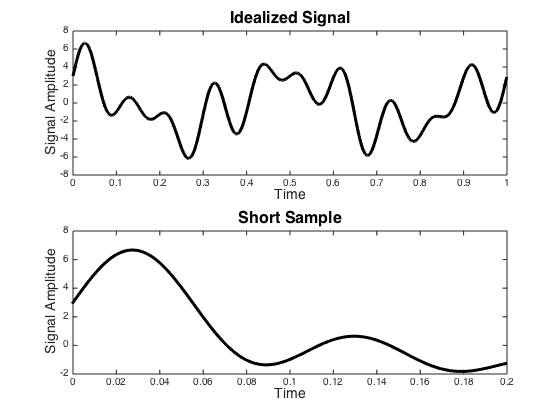
\includegraphics[scale = 0.8]{Figures/idealsig_shortsample.png}
\caption{Plot of ideal sample in the time domain as well as a small sample size that corresponds to 20\% of the total sample size.}
\label{fig:idealsig}
\end{figure}

\begin{figure}[H]
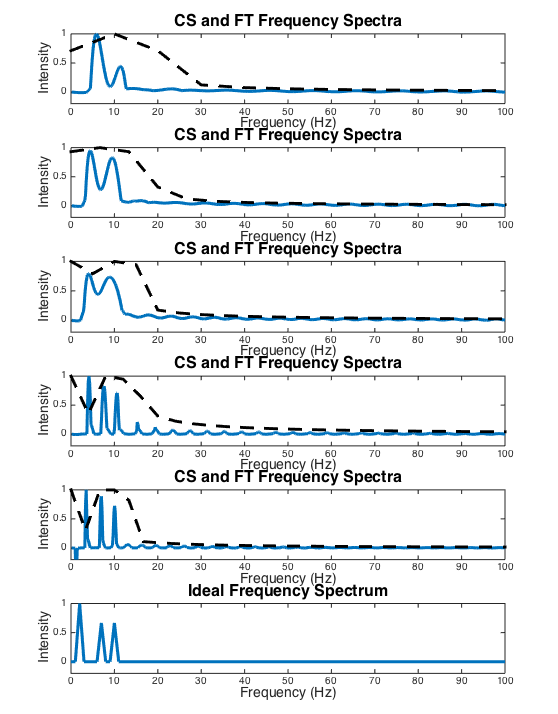
\includegraphics[scale = 0.7]{Figures/samplingtimes_ideal_test.png}
\caption{The black dashed line represents the Fourier transform of the small sample size of the ideal signal while the solid blue line shows the recreated spectrum using the CS technique. The plots, from top to bottom, represent using 5, 10, 15, 20, and 25\% of the full data set, while the Fourier transform of the ideal signal is shown at the bottom.}
\label{fig:idealsamplerates}
\end{figure}
\pagebreak

% SIMULATED CASES

\subsection*{B.	Simulated Optical Absorption Spectra Cases}

\begin{figure}[H]
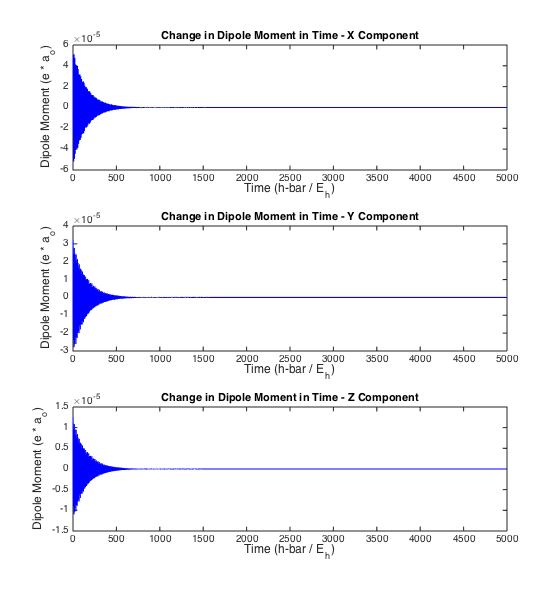
\includegraphics[scale = 0.7]{Figures/fulldipolemoment.png}
\caption{Simulated data showing the oscillating dipole moment in 3 dimensions. Units are in atomic units, where time is shown as $\hbar / E_h$, corresponding to the SI units of seconds.}
\label{fig:fulldipole}
\end{figure}

\begin{figure}[H]
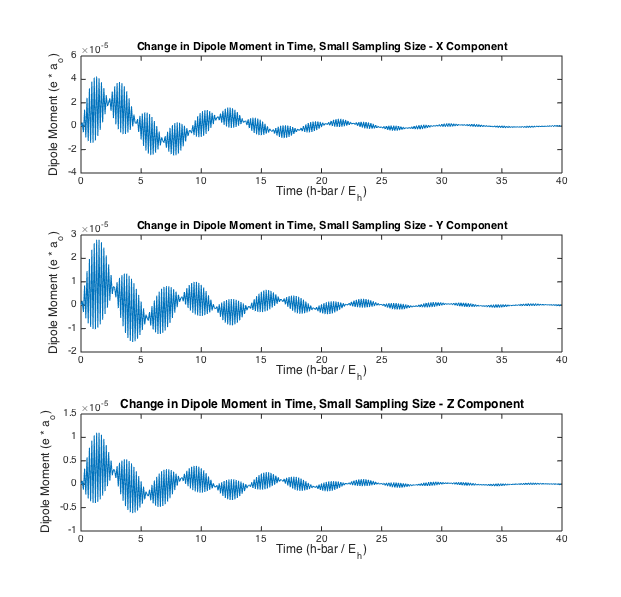
\includegraphics[scale = 0.7]{Figures/dipole_smallsample.png}
\caption{Oscillating dipole moment in 3 dimensions of a small sampling size of the full data. These plots show 400 of the 50,000 time steps of data.}
\label{fig:partdipole}
\end{figure}

\begin{figure}[H]
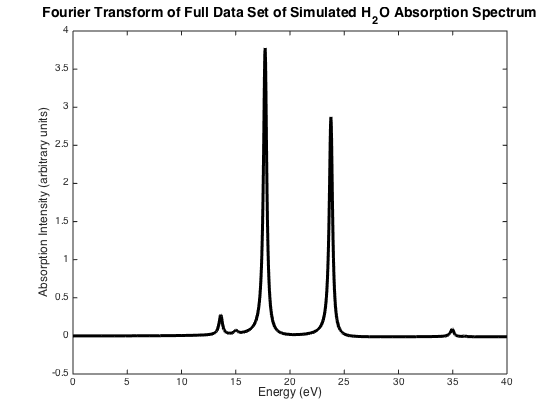
\includegraphics[scale = 0.8]{Figures/ftoffulldata.png}
\caption{Fourier transform of the full 50,000 point data set of the simulated absorption spectrum of water.}
\label{fig:fullFT}
\end{figure}

\begin{figure}[H]
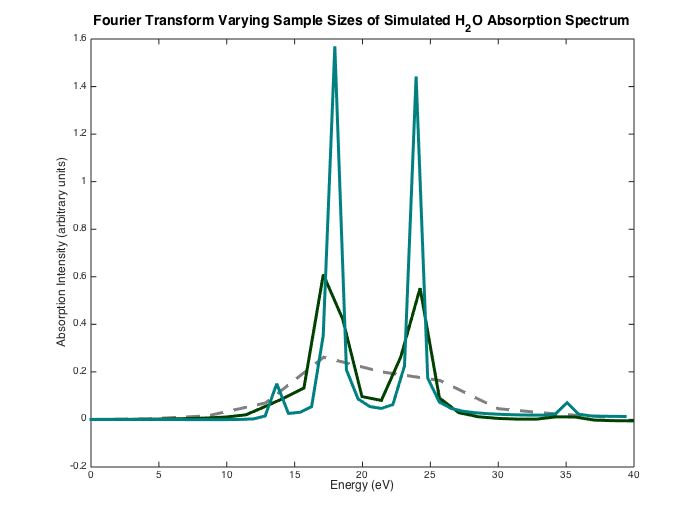
\includegraphics[scale = 0.6]{Figures/FT_comp.png}
\caption{Comparison of the Fourier transform of three sampling sizes of the simulated absorption data set. The gray dashed line represents the transform of 400 points (0.8\%), the dark green line represents 1200 points (2.4\%), and the turquoise line represents the transform of 2000 points (4\%).}
\label{fig:FTcomp}
\end{figure}

\begin{figure}[H]
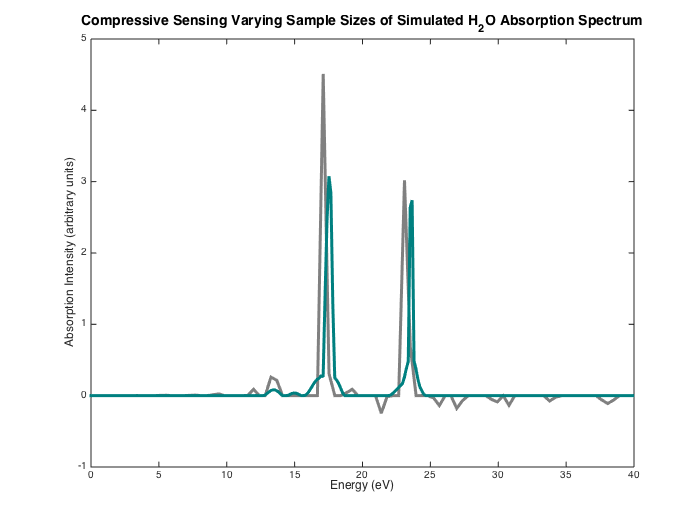
\includegraphics[scale = 0.6]{Figures/CS_comp.png}
\caption{Comparison of the compressing sensing technique applied to two different sampling sizes of the simulated absorption data set. The gray line represents a sampling size of 400 points (0.8\%), the dark green line represents 1200 points (2.4\%).}
\label{fig:CScomp}
\end{figure}

\begin{figure}[H]
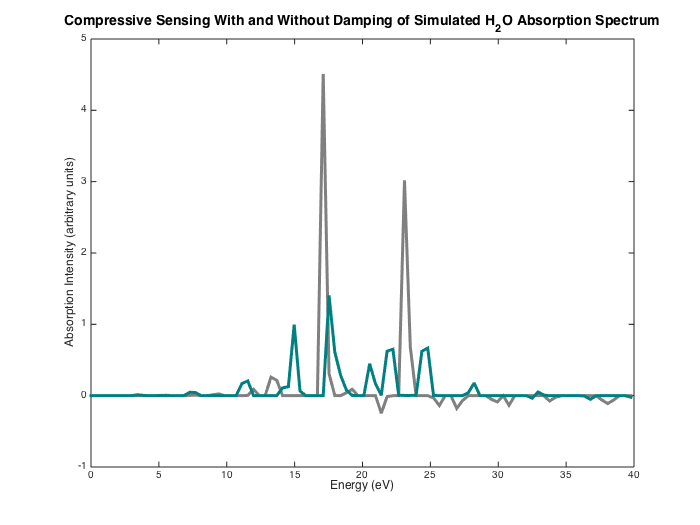
\includegraphics[scale = 0.6]{Figures/wandwodamping.png}
\caption{Comparison of compressed sensing with high and low amount of damping. The green trace is with a high amount of damping (damping constant $\tau$ set to 1500) and the gray trace was with low damping ($\tau$ set to 15).}
\end{figure}

\pagebreak


%SECTION V. -- SUMMARY AND CONCLUSIONS
%We need to be sure to include our comparison of transforms and sampling rates with some sort of
%visualization in this section.  

\section*{V.	Summary and Conclusions} %J with input from Joe and Shichao 

\par As shown above, the compressed sensing technique was able to capture the absorption spectrum to a least semi-quantitative accuracy. In practice this is good enough for most applications. This has profound implications for the computational chemistry community as it allows for highly accurate calculations to be run for a shorter period of time without sacrificing much in the quality of results.\\ 

Our tests above utilized the SPGL1 basis pursuit method due to its speed advantage over other L1 minimization algorithms such as CVX. However, other possible methods for further reducing the time of calculation include running a coarse calculation first to determine key windows of interest, followed by a second fine-grained spectra (artificially setting some of the rows in the Fourier matrix to zero). Additionally, while this implementation of compressed sensing was carried out in the MATLAB environment, much of our group workflow uses Python and associated SciPy packages. Porting the scripts to Python would facilitate quick analysis that is more automated and less prone to error.\\

Finally, since we were able to demonstrate a useful signal reconstruction using CS, this technique may now be applied as an option in our RT-TDDFT program.  This would reduce the simulation run time requirement for resolving the features of interest in simulated spectra.\\ 


\pagebreak

% BIBLIOGRAPHY -----------------------------------------------------------------------------------------
\begin{thebibliography}{9}
\setlength{\itemsep}{-2mm}\footnotesize{

\bibitem{Andrade} X. Andrade, J. N. Sanders, and A. Aspuru-Guzik, \textit{Application of compressed sensing to the simulation of atomic systems,} PNAS. Vol 109 (2012) pp. 12938-13933.

\bibitem{Kutz} J. N. Kutz, \textit{Ch. 17 Basics of Compressed Sensing,} AMATH 582 Course Notes. (2016). pp. 395-418.

\bibitem{vandenBerg} E. van den Berg and M. P. Friedlander, \textit{Probing the Pareto frontier basis pursuit solutions,}

}\end{thebibliography}

\pagebreak
%APPENDICES-----------------------------------------------------------------------------------------------

\begin{appendices}

\section{MATLAB Functions and Implementations}

\subsection*{fft}

\subsection*{fftshift}

\subsection*{csvread}

\subsection*{spg\_bpdn}

\subsection*{spg\_bp}

\subsection*{find}

\subsection*{toc}

% MATLAB CODE SECTION ------------------------------------------------------------------------------
\section{MATLAB Code}
First, we have the script \emph{compressed\_sensing} which manipulates the idealized case from \emph{Part One}:\\
\begin{verbatim}
%Compressed Sensing
%AMATH 582 Final Project
%J. Kasper, C. Houferak, J. Radler, S. Sun

%% Step 1: Known Signal
clc;
clear;
N = 2000; %total time length (ENTIRE signal)
t2 = linspace(0,1,N+1); t=t2(1:N);

S = 2*sin(10*t*(2*pi))+2*sin(7*t*(2*pi))+3*cos(2*t*(2*pi)); %idealized signal

n=400; %number of points to sample
samp = S(1:n)';

figure(1)
subplot(2,1,1)
plot(t,S)
xlabel('Time')
ylabel('Signal Amplitude')
title('Idealized Signal')

subplot(2,1,2)
plot(t(1:n),samp)
xlabel('Time')
ylabel('Signal Amplitude')
title('Short Sample')

deltaOmega = t(N)-t(1); %frequency difference

%generate Discrete Sine matrix
for j = 1:n
    for k = 1:N
        F(j,k) = (2/pi)*deltaOmega*sin(j*t(k));
    end
end

%solve the equation F*x = samp
sigma = 0.05;
opts = spgSetParms('verbosity',0);         % Turn off the SPGL1 log output
x = spg_bpdn(F, samp, sigma, opts);

%check if the error is small
norm(samp-F*x)

%reconstruct the signal from CS coefficients
csSignal = zeros(size(t));
for i = 1:N
    csSignal = csSignal + sin(deltaOmega*t*i)*x(i);
end

figure(2)
plot(t,csSignal)
xlabel('Time')
ylabel('Signal Amplitude')
title('Compressed Sensing Signal')


x = x/max(abs(x)); %normalize

St2 = abs(fftshift(fft(S)));
St = St2(N/2+1:N)/max(St2); %take the last half (positive frequencies)

sampt2 = abs(fftshift(fft(samp)));
sampt = sampt2(n/2:n)/max(sampt2);

%frequency domain for CS signal
for i = 1:length(t)
    freq(i) = i/(2*pi);
end

%frequency domain for entire signal
for i = 1:length(St)
    freq2(i) = i-1;
end

%frequency domain for Fourier transformed sample
for i = 1:length(sampt)
    freq3(i) = (N/n)*(i-1);
end


figure(3)
hold on
subplot(3,1,1), plot(freq2,St);
title('Ideal Frequency Spectrum')
xlabel('Frequency (Hz)')
ylabel('Normalized Intensity')
axis([0 100 -.2 1])
subplot(3,1,2), plot(freq,x)
title('Compressed Sensing Frequency Spectrum')
xlabel('Frequency (Hz)')
ylabel('Normalized Intensity')
axis([0 100 -.2 1])
subplot(3,1,3), plot(freq3,sampt)
title('Fourier Transform Frequency Spectrum')
xlabel('Frequency (Hz)')
ylabel('Normalized Intensity')
axis([0 100 -.2 1])
hold off
\end{verbatim}

\par Next we have the code for applying CS to simulated optical absorption spectra of water calculated with RT-TDDFT:

\begin{verbatim}
x=csvread('h2o_x_RealTime_Dipole.csv',1,0);
y=csvread('h2o_y_RealTime_Dipole.csv',1,0);
z=csvread('h2o_z_RealTime_Dipole.csv',1,0);
% read the data of dipole moment
 

tic
nn=6000;            % number of data points (long edge of F matrix)
t=x(1:nn,1);        % time
m=fix(nn/5);          %number of used data points  (short edge of F matrix)

T=t(nn);           %simulated simulation time. actual simulation time will be T/5.
dt=t(2)-t(1);       % time step
w=(pi/T)*[0:nn-1];  % frequency
kick=0.0001;        % amplitude of electric field E 

 

 
pxt=x(1:m,3);       
pyt=y(1:m,4);
pzt=z(1:m,5);
% pick the data of angular momentum
 
damp_const=150;
damp = exp(-(t(1:m)-t(1))/damp_const);

 
px=pxt-pxt(1);
py=pyt-pyt(1);
pz=pzt-pzt(1);
% subtract mean value

px=px.*damp;
py=py.*damp;
pz=pz.*damp;

% damp

%change to atomic unit
px=0.393456*px;
py=0.393456*py;
pz=0.393456*py;

 %% 
% do L1 optimization
opts = spgSetParms('verbosity',0); 
FF=idst(eye(nn,nn));
F=FF(1:m,:);
 
ax  = spg_bp(F,px,opts); 

ay  = spg_bp(F,py,opts); 

az  = spg_bp(F,pz,opts); 
%%
 
sigma=(4*pi/(3*137*kick))*w'.*(ax+ay+az);  % sigma=blabla*(axx+ayy+azz)

 
w=27.2114*w;                               %change frequency w into eq
number=find(w<40);                         % confine the w to the frequency interval of we want
np=length(number);                         
figure (2)
plot(w(1:np),sigma(1:np))
toc
\end{verbatim}

%\section{Custom MATLAB Functions} 	%Use subsections for each one

%\subsection*{Custom MATLAB Function 1}

\end{appendices}

\end{document}  
